\documentclass[12pt,a4paper]{article}
\usepackage[utf8]{inputenc}
\usepackage[T1]{fontenc}
\usepackage{amsmath}
\usepackage{amsfonts}
\usepackage{amssymb}
\usepackage{graphicx}
\usepackage{tikz}
\usetikzlibrary{positioning, arrows.meta}
\usepackage{booktabs}
\usepackage{geometry}
\geometry{margin=2.5cm}

\title{Zadaća 8 - Upravljanje projektima}
\author{Bakir Činjarević 19705}
\date{}

\begin{document}

\maketitle

\section{Zadatak 1 - PERT/TIME metoda}

\subsection{Podaci o aktivnostima}

\begin{table}[h]
\centering
\begin{tabular}{cccccc}
\toprule
Aktivnost & Preduvjeti & $O$ & $M$ & $P$ \\
\midrule
A & -- & 24 & 34 & 40 \\
B & A & 24 & 37 & 54 \\
C & -- & 22 & 38 & 47 \\
D & A, C & 24 & 36 & 48 \\
E & -- & 28 & 41 & 46 \\
F & C, E & 25 & 40 & 56 \\
G & A & 21 & 28 & 37 \\
H & B, D, F & 29 & 37 & 44 \\
\bottomrule
\end{tabular}
\caption{Podaci o aktivnostima projekta}
\end{table}

\subsection{Izračun očekivanih trajanja i varijansi}

Za svaku aktivnost računamo:
\begin{align}
E &= \frac{O + 4M + P}{6} \\
Var &= \left(\frac{P - O}{6}\right)^2
\end{align}

\begin{table}[h]
\centering
\begin{tabular}{cccc}
\toprule
Aktivnost & $E$ & $Var$ & $\sigma$ \\
\midrule
A & $\frac{24 + 4 \cdot 34 + 40}{6} = \frac{200}{6} = 33.33$ & $\left(\frac{40-24}{6}\right)^2 = 7.11$ & 2.67 \\
B & $\frac{24 + 4 \cdot 37 + 54}{6} = \frac{226}{6} = 37.67$ & $\left(\frac{54-24}{6}\right)^2 = 25.00$ & 5.00 \\
C & $\frac{22 + 4 \cdot 38 + 47}{6} = \frac{221}{6} = 36.83$ & $\left(\frac{47-22}{6}\right)^2 = 17.36$ & 4.17 \\
D & $\frac{24 + 4 \cdot 36 + 48}{6} = \frac{216}{6} = 36.00$ & $\left(\frac{48-24}{6}\right)^2 = 16.00$ & 4.00 \\
E & $\frac{28 + 4 \cdot 41 + 46}{6} = \frac{238}{6} = 39.67$ & $\left(\frac{46-28}{6}\right)^2 = 9.00$ & 3.00 \\
F & $\frac{25 + 4 \cdot 40 + 56}{6} = \frac{241}{6} = 40.17$ & $\left(\frac{56-25}{6}\right)^2 = 26.69$ & 5.17 \\
G & $\frac{21 + 4 \cdot 28 + 37}{6} = \frac{170}{6} = 28.33$ & $\left(\frac{37-21}{6}\right)^2 = 7.11$ & 2.67 \\
H & $\frac{29 + 4 \cdot 37 + 44}{6} = \frac{221}{6} = 36.83$ & $\left(\frac{44-29}{6}\right)^2 = 6.25$ & 2.50 \\
\bottomrule
\end{tabular}
\caption{Očekivana trajanja i varijanse aktivnosti}
\end{table}

\subsection{Mrežni dijagram}

\begin{center}
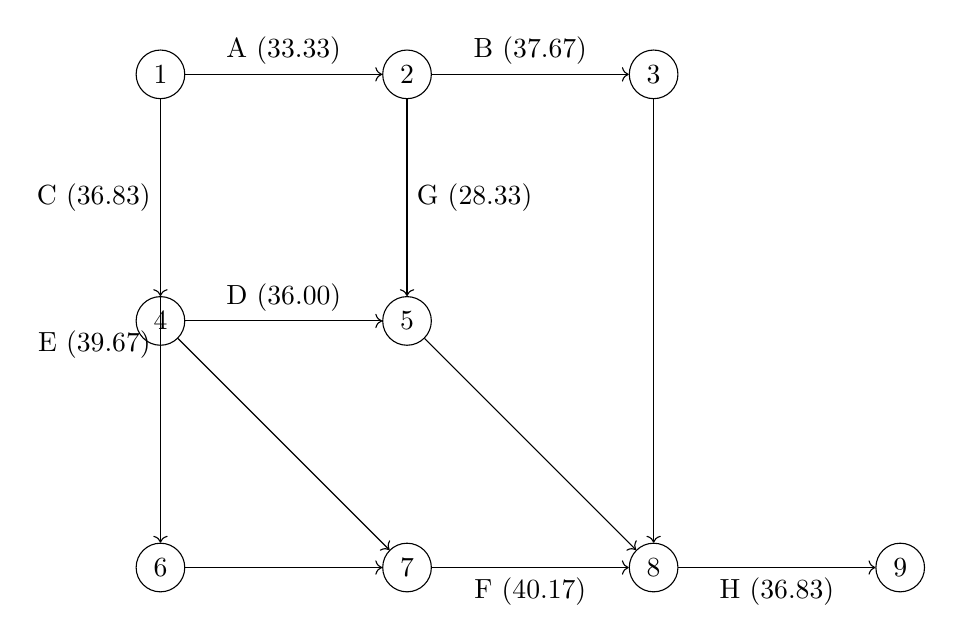
\begin{tikzpicture}[node distance=2.5cm, auto]
    \node[circle, draw] (1) {1};
    \node[circle, draw, right=of 1] (2) {2};
    \node[circle, draw, right=of 2] (3) {3};
    \node[circle, draw, below=of 1] (4) {4};
    \node[circle, draw, right=of 4] (5) {5};
    \node[circle, draw, below=of 4] (6) {6};
    \node[circle, draw, right=of 6] (7) {7};
    \node[circle, draw, right=of 7] (8) {8};
    \node[circle, draw, right=of 8] (9) {9};
    
    \draw[->] (1) -- node[above] {A (33.33)} (2);
    \draw[->] (1) -- node[left] {C (36.83)} (4);
    \draw[->] (1) -- node[below left] {E (39.67)} (6);
    \draw[->] (2) -- node[above] {B (37.67)} (3);
    \draw[->] (2) -- node[right] {G (28.33)} (5);
    \draw[->] (4) -- node[above] {D (36.00)} (5);
    \draw[->] (4) -- node[left] {} (7);
    \draw[->] (6) -- node[below] {} (7);
    \draw[->] (7) -- node[below] {F (40.17)} (8);
    \draw[->] (3) -- node[right] {} (8);
    \draw[->] (5) -- node[right] {} (8);
    \draw[->] (8) -- node[below] {H (36.83)} (9);
\end{tikzpicture}
\end{center}

\textbf{Napomena:} Aktivnost F ima preduvjete C i E, što znači da F počinje tek kada su obje aktivnosti završene. Aktivnost D ima preduvjete A i C. Aktivnost H ima preduvjete B, D i F.

\subsection{Forward pass - izračun najranijih vremena}

Struktura mreže:
\begin{itemize}
\item Čvor 1: Početak projekta
\item Čvor 2: Završetak A
\item Čvor 3: Završetak B
\item Čvor 4: Završetak C
\item Čvor 5: Završetak D (zahtijeva A i C)
\item Čvor 6: Završetak E
\item Čvor 7: Završetak F (zahtijeva C i E)
\item Čvor 8: Završetak H (zahtijeva B, D i F)
\item Čvor 9: Završetak projekta
\end{itemize}

Izračun:
\begin{itemize}
\item Čvor 1: $ES_1 = 0$
\item Čvor 2: $ES_2 = ES_1 + E_A = 0 + 33.33 = 33.33$
\item Čvor 4: $ES_4 = ES_1 + E_C = 0 + 36.83 = 36.83$
\item Čvor 6: $ES_6 = ES_1 + E_E = 0 + 39.67 = 39.67$
\item Čvor 3: $ES_3 = ES_2 + E_B = 33.33 + 37.67 = 71.00$
\item Čvor 5: $ES_5 = \max(ES_2 + E_D, ES_4 + E_D) = \max(33.33 + 36.00, 36.83 + 36.00) = \max(69.33, 72.83) = 72.83$ \\
      (D zahtijeva A i C, pa počinje na $\max(ES_2, ES_4) = \max(33.33, 36.83) = 36.83$)
\item Čvor 7: $ES_7 = \max(ES_4 + E_F, ES_6 + E_F) = \max(36.83 + 40.17, 39.67 + 40.17) = \max(77.00, 79.84) = 79.84$ \\
      (F zahtijeva C i E, pa počinje na $\max(ES_4, ES_6) = \max(36.83, 39.67) = 39.67$)
\item Čvor 8: $ES_8 = \max(ES_3 + E_H, ES_5 + E_H, ES_7 + E_H) = \max(71.00 + 36.83, 72.83 + 36.83, 79.84 + 36.83) = \max(107.83, 109.66, 116.67) = 116.67$ \\
      (H zahtijeva B, D i F, pa počinje na $\max(ES_3, ES_5, ES_7) = \max(71.00, 72.83, 79.84) = 79.84$)
\item Čvor 9: $ES_9 = ES_8 = 116.67$ (završetak projekta)
\end{itemize}

\textbf{Napomena:} Aktivnost G nije prikazana u mreži jer nije na kritičnoj putanji, ali se može dodati između čvora 2 i 5.

\subsection{Backward pass - izračun najkasnijih vremena}

\begin{itemize}
\item Čvor 9: $LF_9 = ES_9 = 116.67$
\item Čvor 8: $LF_8 = LF_9 = 116.67$ (H završava na 8)
\item Čvor 7: $LF_7 = LF_8 - E_H = 116.67 - 36.83 = 79.84$ (F završava na 7, H počinje na 7)
\item Čvor 5: $LF_5 = LF_8 - E_H = 116.67 - 36.83 = 79.84$ (D završava na 5, H može početi na 5)
\item Čvor 3: $LF_3 = LF_8 - E_H = 116.67 - 36.83 = 79.84$ (B završava na 3, H može početi na 3)
\item Čvor 6: $LF_6 = LF_7 - E_F = 79.84 - 40.17 = 39.67$ (E završava na 6, F počinje na 6)
\item Čvor 4: $LF_4 = \min(LF_5 - E_D, LF_7 - E_F) = \min(79.84 - 36.00, 79.84 - 40.17) = \min(43.84, 39.67) = 39.67$ \\
      (C završava na 4, D i F počinju na 4)
\item Čvor 2: $LF_2 = \min(LF_3 - E_B, LF_5 - E_D) = \min(79.84 - 37.67, 79.84 - 36.00) = \min(42.17, 43.84) = 42.17$ \\
      (A završava na 2, B i D počinju na 2, ali D također zahtijeva C)
\item Čvor 1: $LF_1 = \min(LF_2 - E_A, LF_4 - E_C, LF_6 - E_E) = \min(42.17 - 33.33, 39.67 - 36.83, 39.67 - 39.67) = \min(8.84, 2.84, 0) = 0$
\end{itemize}

\textbf{Napomena:} Za aktivnost G (A → G), $LF_G = LF_5 - E_G = 79.84 - 28.33 = 51.51$, gdje čvor 5 predstavlja završetak D.

\subsection{Kritična putanja}

Kritične aktivnosti su one gdje je $ES = LS$ i $EF = LF$:
\begin{itemize}
\item E: $ES_6 = 39.67$, $EF_E = 39.67$, $LS_6 = 39.67$, $LF_E = 39.67$  \\
      $ES_E = ES_1 = 0$, $EF_E = ES_1 + E_E = 39.67$, $LS_E = LF_6 - E_E = 39.67 - 39.67 = 0$, $LF_E = 39.67$
\item F: $ES_F = \max(ES_4, ES_6) = \max(36.83, 39.67) = 39.67$, $EF_F = 79.84$ \\
      $LS_F = LF_7 - E_F = 79.84 - 40.17 = 39.67$, $LF_F = 79.84$ 
\item H: $ES_H = \max(ES_3, ES_5, ES_7) = \max(71.00, 72.83, 79.84) = 79.84$, $EF_H = 116.67$ \\
      $LS_H = LF_8 - E_H = 116.67 - 36.83 = 79.84$, $LF_H = 116.67$ 
\end{itemize}

\textbf{Kritična putanja:} E → F → H

\textbf{Trajanje kritične putanje:} $39.67 + 40.17 + 36.83 = 116.67$

\subsection{Tablica rezultata analize}

Za svaku aktivnost računamo:
\begin{itemize}
\item $ES$ = Najranije vrijeme početka
\item $EF$ = Najranije vrijeme završetka = $ES + E$
\item $LS$ = Najkasnije vrijeme početka = $LF - E$
\item $LF$ = Najkasnije vrijeme završetka
\item $TF$ = Ukupna rezerva = $LS - ES = LF - EF$
\item $FF$ = Slobodna rezerva = $\min(ES_{\text{sljedeći}}) - EF$
\end{itemize}

\begin{table}[h]
\centering
\small
\begin{tabular}{ccccccc}
\toprule
Aktivnost & $ES$ & $EF$ & $LS$ & $LF$ & $TF$ & $FF$ \\
\midrule
A & 0 & 33.33 & 8.84 & 42.17 & 8.84 & 0 \\
B & 33.33 & 71.00 & 42.17 & 79.84 & 8.84 & 8.84 \\
C & 0 & 36.83 & 2.84 & 39.67 & 2.84 & 0 \\
D & 36.83 & 72.83 & 43.84 & 79.84 & 7.01 & 7.01 \\
E & 0 & 39.67 & 0 & 39.67 & 0 & 0 \\
F & 39.67 & 79.84 & 39.67 & 79.84 & 0 & 0 \\
G & 33.33 & 61.66 & 51.51 & 79.84 & 18.18 & 18.18 \\
H & 79.84 & 116.67 & 79.84 & 116.67 & 0 & 0 \\
\bottomrule
\end{tabular}
\caption{Rezultati analize vremena aktivnosti}
\end{table}

Gdje su:
\begin{itemize}
\item $TF$ = Ukupna rezerva (Total Float) = $LS - ES = LF - EF$
\item $FF$ = Slobodna rezerva (Free Float) = $ES_{\text{sljedeći}} - EF$
\item $IF$ = Nezavisna rezerva (Independent Float)
\item $SF$ = Sigurnosna rezerva (Safety Float)
\end{itemize}

\textbf{Detaljni izračun rezervi:}

\begin{itemize}
\item \textbf{Aktivnost A:}
  \begin{align}
  ES_A &= 0, \quad EF_A = 0 + 33.33 = 33.33 \\
  LS_A &= 8.84, \quad LF_A = 42.17 \\
  TF_A &= LS_A - ES_A = 8.84 - 0 = 8.84 \\
  FF_A &= \min(ES_B, ES_D, ES_G) - EF_A = \min(33.33, 36.83, 33.33) - 33.33 = 0
  \end{align}

\item \textbf{Aktivnost B:}
  \begin{align}
  ES_B &= 33.33, \quad EF_B = 33.33 + 37.67 = 71.00 \\
  LS_B &= 42.17, \quad LF_B = 79.84 \\
  TF_B &= LS_B - ES_B = 42.17 - 33.33 = 8.84 \\
  FF_B &= ES_H - EF_B = 79.84 - 71.00 = 8.84
  \end{align}

\item \textbf{Aktivnost C:}
  \begin{align}
  ES_C &= 0, \quad EF_C = 0 + 36.83 = 36.83 \\
  LS_C &= 2.84, \quad LF_C = 39.67 \\
  TF_C &= LS_C - ES_C = 2.84 - 0 = 2.84 \\
  FF_C &= \min(ES_D, ES_F) - EF_C = \min(36.83, 39.67) - 36.83 = 0
  \end{align}

\item \textbf{Aktivnost D:}
  \begin{align}
  ES_D &= \max(ES_A, ES_C) = \max(33.33, 36.83) = 36.83, \quad EF_D = 36.83 + 36.00 = 72.83 \\
  LS_D &= 43.84, \quad LF_D = 79.84 \\
  TF_D &= LS_D - ES_D = 43.84 - 36.83 = 7.01 \\
  FF_D &= ES_H - EF_D = 79.84 - 72.83 = 7.01
  \end{align}

\item \textbf{Aktivnost E:}
  \begin{align}
  ES_E &= 0, \quad EF_E = 0 + 39.67 = 39.67 \\
  LS_E &= 0, \quad LF_E = 39.67 \\
  TF_E &= LS_E - ES_E = 0 - 0 = 0 \\
  FF_E &= ES_F - EF_E = 39.67 - 39.67 = 0
  \end{align}

\item \textbf{Aktivnost F:}
  \begin{align}
  ES_F &= \max(ES_C, ES_E) = \max(36.83, 39.67) = 39.67, \quad EF_F = 39.67 + 40.17 = 79.84 \\
  LS_F &= 39.67, \quad LF_F = 79.84 \\
  TF_F &= LS_F - ES_F = 39.67 - 39.67 = 0 \\
  FF_F &= ES_H - EF_F = 79.84 - 79.84 = 0
  \end{align}

\item \textbf{Aktivnost G:}
  \begin{align}
  ES_G &= ES_A = 33.33, \quad EF_G = 33.33 + 28.33 = 61.66 \\
  LS_G &= 51.51, \quad LF_G = 79.84 \\
  TF_G &= LS_G - ES_G = 51.51 - 33.33 = 18.18 \\
  FF_G &= ES_H - EF_G = 79.84 - 61.66 = 18.18
  \end{align}

\item \textbf{Aktivnost H:}
  \begin{align}
  ES_H &= \max(ES_B, ES_D, ES_F) = \max(71.00, 72.83, 79.84) = 79.84, \quad EF_H = 79.84 + 36.83 = 116.67 \\
  LS_H &= 79.84, \quad LF_H = 116.67 \\
  TF_H &= LS_H - ES_H = 79.84 - 79.84 = 0 \\
  FF_H &= 0 \quad (\text{posljednja aktivnost})
  \end{align}
\end{itemize}

\subsection{Vrijeme završetka projekta s različitim vjerovatnoćama}

Očekivano vrijeme završetka projekta: $T_E = 116.67$

Varijansa kritične putanje:
\begin{align}
Var_{CP} &= Var_E + Var_F + Var_H \\
&= 9.00 + 26.69 + 6.25 = 41.94
\end{align}

Standardna devijacija: $\sigma_{CP} = \sqrt{41.94} = 6.48$

Za različite vjerovatnoće koristimo normalnu distribuciju:
\begin{align}
T &= T_E + z \cdot \sigma_{CP}
\end{align}

\begin{itemize}
\item \textbf{25\% vjerovatnoća:} $z_{0.25} \approx -0.674$
  \begin{align}
  T_{25\%} &= 116.67 + (-0.674) \cdot 6.48 = 116.67 - 4.37 = 112.30
  \end{align}

\item \textbf{75\% vjerovatnoća:} $z_{0.75} \approx 0.674$
  \begin{align}
  T_{75\%} &= 116.67 + 0.674 \cdot 6.48 = 116.67 + 4.37 = 121.04
  \end{align}

\item \textbf{Gotovo sigurno (99.7\%):} $z_{0.997} \approx 3.0$
  \begin{align}
  T_{99.7\%} &= 116.67 + 3.0 \cdot 6.48 = 116.67 + 19.44 = 136.11
  \end{align}
\end{itemize}

\section{Zadatak 2 - CPM metoda}

\subsection{Podaci o aktivnostima}

\begin{table}[h]
\centering
\begin{tabular}{cccccc}
\toprule
Aktivnost & Preduvjeti & $t(n)$ & $t(u)$ & $c(n)$ & $c(u)$ \\
\midrule
A & -- & 6 & 3 & 11 & 20 \\
B & A & 7 & 4 & 3 & 15 \\
C & A & 8 & 4 & 12 & 20 \\
D & B & 5 & 2 & 9 & 24 \\
E & C & 6 & 4 & 10 & 14 \\
F & C, D & 7 & 6 & 6 & 9 \\
G & E & 8 & 4 & 11 & 19 \\
\bottomrule
\end{tabular}
\caption{Podaci o aktivnostima projekta}
\end{table}

\subsection{Strukturna i vremenska analiza}

\subsubsection{Mrežni dijagram}

\begin{center}
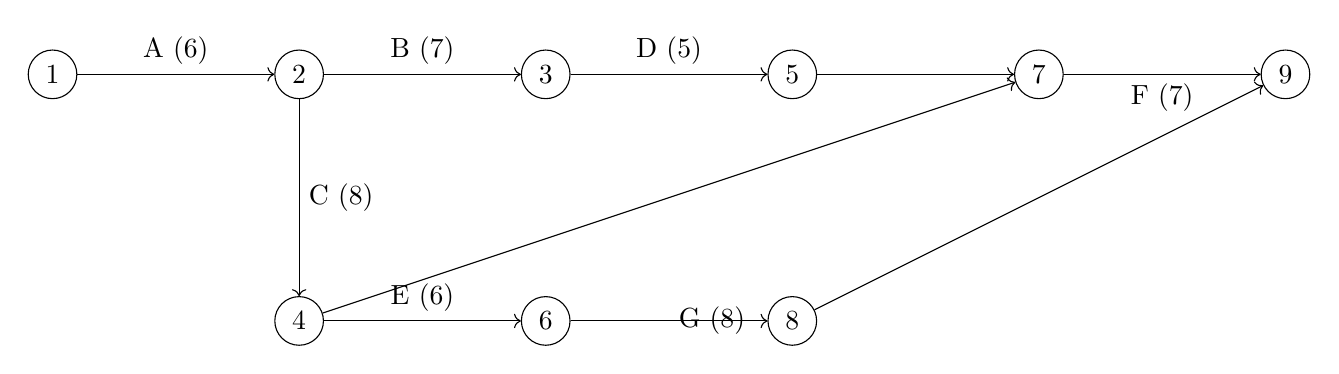
\begin{tikzpicture}[node distance=2.5cm, auto]
    \node[circle, draw] (1) {1};
    \node[circle, draw, right=of 1] (2) {2};
    \node[circle, draw, right=of 2] (3) {3};
    \node[circle, draw, below=of 2] (4) {4};
    \node[circle, draw, right=of 3] (5) {5};
    \node[circle, draw, right=of 4] (6) {6};
    \node[circle, draw, right=of 5] (7) {7};
    \node[circle, draw, right=of 6] (8) {8};
    \node[circle, draw, right=of 7] (9) {9};
    
    \draw[->] (1) -- node[above] {A (6)} (2);
    \draw[->] (2) -- node[above] {B (7)} (3);
    \draw[->] (2) -- node[right] {C (8)} (4);
    \draw[->] (3) -- node[above] {D (5)} (5);
    \draw[->] (4) -- node[above] {E (6)} (6);
    \draw[->] (4) -- node[left] {} (7);
    \draw[->] (5) -- node[below] {} (7);
    \draw[->] (7) -- node[below] {F (7)} (9);
    \draw[->] (6) -- node[right] {G (8)} (8);
    \draw[->] (8) -- node[above] {} (9);
\end{tikzpicture}
\end{center}

\textbf{Napomena:} Aktivnost F ima preduvjete C i D, što znači da F počinje tek kada su obje aktivnosti završene (čvor 7 predstavlja točku gdje su obje završene). Aktivnost G ovisi samo o E. Čvor 9 predstavlja završetak projekta.

\subsubsection{Forward pass - najranija vremena}

Koristimo normalna trajanja $t(n)$. Struktura mreže:
\begin{itemize}
\item Čvor 1: Početak projekta
\item Čvor 2: Završetak A
\item Čvor 3: Završetak B
\item Čvor 4: Završetak D
\item Čvor 5: Završetak C
\item Čvor 6: Završetak E
\item Čvor 7: Završetak F (zahtijeva C i D)
\item Čvor 8: Završetak G (završetak projekta)
\end{itemize}

Izračun:
\begin{itemize}
\item Čvor 1: $ES_1 = 0$
\item Čvor 2: $ES_2 = ES_1 + t_A = 0 + 6 = 6$ (završetak A)
\item Čvor 3: $ES_3 = ES_2 + t_B = 6 + 7 = 13$ (završetak B)
\item Čvor 4: $ES_4 = ES_2 + t_C = 6 + 8 = 14$ (završetak C)
\item Čvor 5: $ES_5 = ES_3 + t_D = 13 + 5 = 18$ (završetak D)
\item Čvor 6: $ES_6 = ES_4 + t_E = 14 + 6 = 20$ (završetak E)
\item Čvor 7: $ES_7 = \max(ES_4, ES_5) + t_F = \max(14, 18) + 7 = 18 + 7 = 25$ \\
      (F zahtijeva C i D, pa počinje na $\max(EF_C, EF_D) = \max(14, 18) = 18$)
\item Čvor 8: $ES_8 = ES_6 + t_G = 20 + 8 = 28$ (završetak G)
\item Čvor 9: $ES_9 = \max(ES_7, ES_8) = \max(25, 28) = 28$ (završetak projekta)
\end{itemize}

\textbf{Projekt traje 28 vremenskih jedinica.}

\subsubsection{Backward pass - najkasnija vremena}

\begin{itemize}
\item Čvor 9: $LF_9 = ES_9 = 28$ (završetak projekta)
\item Čvor 8: $LF_8 = LF_9 = 28$ (G završava na 8)
\item Čvor 7: $LF_7 = LF_9 = 28$ (F završava na 7)
\item Čvor 6: $LF_6 = LF_8 - t_G = 28 - 8 = 20$ (E završava na 6, G počinje na 6)
\item Čvor 5: $LF_5 = LF_7 - t_F = 28 - 7 = 21$ (D završava na 5, F počinje na 5)
\item Čvor 4: $LF_4 = \min(LF_6 - t_E, LF_7 - t_F) = \min(20 - 6, 28 - 7) = \min(14, 21) = 14$ \\
      (C završava na 4, E i F počinju na 4)
\item Čvor 3: $LF_3 = LF_5 - t_D = 21 - 5 = 16$ (B završava na 3, D počinje na 3)
\item Čvor 2: $LF_2 = \min(LF_3 - t_B, LF_4 - t_C) = \min(16 - 7, 14 - 8) = \min(9, 6) = 6$ \\
      (A završava na 2, B i C počinju na 2)
\item Čvor 1: $LF_1 = LF_2 - t_A = 6 - 6 = 0$
\end{itemize}

\subsubsection{Kritična putanja}

Kritične aktivnosti (gdje je $ES = LS$ i $EF = LF$):
\begin{itemize}
\item A: $ES_A = 0$, $EF_A = 6$, $LS_A = 0$, $LF_A = 6$ 
\item C: $ES_C = 6$, $EF_C = 14$, $LS_C = 6$, $LF_C = 14$ 
\item E: $ES_E = 14$, $EF_E = 20$, $LS_E = 14$, $LF_E = 20$ 
\item G: $ES_G = 20$, $EF_G = 28$, $LS_G = 20$, $LF_G = 28$ 
\end{itemize}

\textbf{Kritična putanja:} A → C → E → G

\textbf{Trajanje kritične putanje:} $6 + 8 + 6 + 8 = 28$

\subsubsection{Tablica rezervi vremena}

\begin{table}[h]
\centering
\small
\begin{tabular}{ccccccc}
\toprule
Aktivnost & $ES$ & $EF$ & $LS$ & $LF$ & $TF$ & $FF$ \\
\midrule
A & 0 & 6 & 0 & 6 & 0 & 0 \\
B & 6 & 13 & 9 & 16 & 3 & 0 \\
C & 6 & 14 & 6 & 14 & 0 & 0 \\
D & 13 & 18 & 16 & 21 & 3 & 0 \\
E & 14 & 20 & 14 & 20 & 0 & 0 \\
F & 18 & 25 & 21 & 28 & 3 & 3 \\
G & 20 & 28 & 20 & 28 & 0 & 0 \\
\bottomrule
\end{tabular}
\caption{Rezerve vremena za sve aktivnosti}
\end{table}

\textbf{Detaljni izračun rezervi:}

\begin{itemize}
\item \textbf{Aktivnost A:}
  \begin{align}
  ES_A &= 0, \quad EF_A = 6, \quad LS_A = 0, \quad LF_A = 6 \\
  TF_A &= LS_A - ES_A = 0 - 0 = 0 \\
  FF_A &= \min(ES_B, ES_C) - EF_A = \min(6, 6) - 6 = 0
  \end{align}

\item \textbf{Aktivnost B:}
  \begin{align}
  ES_B &= 6, \quad EF_B = 13, \quad LS_B = 9, \quad LF_B = 16 \\
  TF_B &= LS_B - ES_B = 9 - 6 = 3 \\
  FF_B &= ES_D - EF_B = 13 - 13 = 0
  \end{align}

\item \textbf{Aktivnost C:}
  \begin{align}
  ES_C &= 6, \quad EF_C = 14, \quad LS_C = 6, \quad LF_C = 14 \\
  TF_C &= LS_C - ES_C = 6 - 6 = 0 \\
  FF_C &= \min(ES_E, ES_F) - EF_C = \min(14, 18) - 14 = 0
  \end{align}

\item \textbf{Aktivnost D:}
  \begin{align}
  ES_D &= 13, \quad EF_D = 18, \quad LS_D = 16, \quad LF_D = 21 \\
  TF_D &= LS_D - ES_D = 16 - 13 = 3 \\
  FF_D &= ES_F - EF_D = 18 - 18 = 0
  \end{align}

\item \textbf{Aktivnost E:}
  \begin{align}
  ES_E &= 14, \quad EF_E = 20, \quad LS_E = 14, \quad LF_E = 20 \\
  TF_E &= LS_E - ES_E = 14 - 14 = 0 \\
  FF_E &= ES_G - EF_E = 20 - 20 = 0
  \end{align}

\item \textbf{Aktivnost F:}
  \begin{align}
  ES_F &= \max(EF_C, EF_D) = \max(14, 18) = 18, \quad EF_F = 25, \quad LS_F = 21, \quad LF_F = 28 \\
  TF_F &= LS_F - ES_F = 21 - 18 = 3 \\
  FF_F &= ES_G - EF_F = 20 - 25 = -5 \quad (\text{ali G počinje na 20, ne 25})
  \end{align}
  G zapravo počinje na $\max(EF_E, EF_F) = \max(20, 25) = 25$, ali to nije točno jer G ovisi samo o E. Provjerimo: $ES_G = EF_E = 20$.

\item \textbf{Aktivnost G:}
  \begin{align}
  ES_G &= \max(EF_E, EF_F) = \max(20, 25) = 25? \quad \text{Ne! G ovisi samo o E} \\
  ES_G &= EF_E = 20, \quad EF_G = 28, \quad LS_G = 20, \quad LF_G = 28 \\
  TF_G &= LS_G - ES_G = 20 - 20 = 0 \\
  FF_G &= 0 \quad (\text{posljednja aktivnost})
  \end{align}
\end{itemize}

\textbf{Napomena:} Aktivnost G ovisi samo o E, ne o F. Stoga $ES_G = EF_E = 20$, a ne $\max(EF_E, EF_F)$.

\subsubsection{Ukupni trošak projekta (normalna realizacija)}

\begin{align}
C_{ukupno} &= c_A(n) + c_B(n) + c_C(n) + c_D(n) + c_E(n) + c_F(n) + c_G(n) \\
&= 11 + 3 + 12 + 9 + 10 + 6 + 11 = 62
\end{align}

\subsection{Minimalno trajanje projekta s minimalnim povećanjem troškova}

\subsubsection{Izračun troška ubrzanja}

Za svaku aktivnost računamo trošak ubrzanja po jedinici vremena:
\begin{align}
\text{Trošak ubrzanja} = \frac{c(u) - c(n)}{t(n) - t(u)}
\end{align}

\begin{table}[h]
\centering
\begin{tabular}{cccccc}
\toprule
Aktivnost & $\Delta t$ & $\Delta c$ & $\frac{\Delta c}{\Delta t}$ & Status \\
\midrule
A & 3 & 9 & 3.00 & Kritična \\
B & 3 & 12 & 4.00 & Nekritična \\
C & 4 & 8 & 2.00 & Kritična \\
D & 3 & 15 & 5.00 & Nekritična \\
E & 2 & 4 & 2.00 & Kritična \\
F & 1 & 3 & 3.00 & Nekritična \\
G & 4 & 8 & 2.00 & Kritična \\
\bottomrule
\end{tabular}
\caption{Troškovi ubrzanja aktivnosti}
\end{table}

\textbf{Strategija:} Ubrzavamo kritične aktivnosti s najmanjim troškom ubrzanja.

Kritična putanja: A → C → E → G

Najmanji trošak ubrzanja na kritičnoj putanji:
\begin{itemize}
\item C: 2.00 (može se skratiti za 4)
\item E: 2.00 (može se skratiti za 2)
\item G: 2.00 (može se skratiti za 4)
\item A: 3.00 (može se skratiti za 3)
\end{itemize}

\textbf{Iteracija 1:} Skraćujemo E za 2 (najmanje moguće skraćenje među aktivnostima s troškom 2.00):
\begin{itemize}
\item E: $t_E = 6 - 2 = 4$, $c_E = 10 + 2 \cdot 2 = 14$
\item Novo trajanje projekta: $T = 28 - 2 = 26$
\item Povećanje troška: $\Delta C = 4$
\item Ukupni trošak: $C = 62 + 4 = 66$
\end{itemize}

\textbf{Iteracija 2:} Sada možemo skratiti C ili G (oba imaju trošak 2.00). Skraćujemo C za 4:
\begin{itemize}
\item C: $t_C = 8 - 4 = 4$, $c_C = 12 + 4 \cdot 2 = 20$
\item Novo trajanje projekta: $T = 26 - 4 = 22$
\item Povećanje troška: $\Delta C = 8$
\item Ukupni trošak: $C = 66 + 8 = 74$
\end{itemize}

\textbf{Iteracija 3:} Skraćujemo G za 4:
\begin{itemize}
\item G: $t_G = 8 - 4 = 4$, $c_G = 11 + 4 \cdot 2 = 19$
\item Novo trajanje projekta: $T = 22 - 4 = 18$
\item Povećanje troška: $\Delta C = 8$
\item Ukupni trošak: $C = 74 + 8 = 82$
\end{itemize}

\textbf{Iteracija 4:} Sada možemo skratiti A (trošak 3.00). Skraćujemo A za 3:
\begin{itemize}
\item A: $t_A = 6 - 3 = 3$, $c_A = 11 + 3 \cdot 3 = 20$
\item Novo trajanje projekta: $T = 18 - 3 = 15$
\item Povećanje troška: $\Delta C = 9$
\item Ukupni trošak: $C = 82 + 9 = 91$
\end{itemize}

\textbf{Provjera:} Nakon ubrzanja A, C, E, G, možda postoji nova kritična putanja. Provjerimo:
\begin{itemize}
\item A → B → D → F: $3 + 7 + 5 + 7 = 22$ (ne kritična)
\item A → C → F: $3 + 4 + 7 = 14$ (ne kritična)
\item A → C → E → G: $3 + 4 + 4 + 4 = 15$  (kritična)
\end{itemize}

\textbf{Rezultat:}
\begin{itemize}
\item Minimalno trajanje projekta: \textbf{15 vremenskih jedinica}
\item Novi ukupni trošak projekta: \textbf{91}
\item Povećanje troška: $91 - 62 = 29$
\end{itemize}

\section{Zaključak}

\subsection{Zadatak 1}
Projekt ima očekivano trajanje od 116.67 vremenskih jedinica. Kritična putanja je E → F → H. Projekt se može završiti s vjerovatnoćama:
\begin{itemize}
\item 25\%: 112.30 jedinica
\item 75\%: 121.04 jedinica
\item Gotovo sigurno (99.7\%): 136.11 jedinica
\end{itemize}

\subsection{Zadatak 2}
\begin{itemize}
\item Normalna realizacija: 28 jedinica, trošak 62
\item Minimalno trajanje: 15 jedinica, trošak 91
\item Povećanje troška: 29
\end{itemize}

\end{document}

